\lecture{1}{Mon 10 Apr 2023 16:33}{final paper}
\newpage
\section*{Abstract}
\addcontentsline{toc}{section}{Abstract}

\begin{adjustwidth}{0.5in}{0.5in}
	This experimental investigation aimed to verify the Compton effect and demonstrate the wave-particle duality of photons using an aluminum rod for electron beam scattering. The collision between a photon and a stationary electron was analyzed, and the Compton effect was derived through energy and momentum conservation principles. The experiment used a setup where photons emitted from an X-ray source collided with a stationary aluminum rod, and the scattered photons were detected by moving detectors positioned at various angles with respect to the incident photons. The resulting histogram illustrated the intensity of scattered photons as a function of the scattering angle. The study found a strong linear relationship between $(1-\cos\theta)$ and $(1/E_{\max})$, supporting the underlying theory of Compton scattering. The experimental value of the rest energy of the electron was determined to be $m_ec^2 = 514 \pm 79$ keV, which is within a 0.5\% relative error from the accepted value of $511$ keV. The study also highlighted the presence of large angular uncertainties due to the lack of precise instrumentation in locating the detector, which could be addressed in future research by employing more accurate instruments to reduce these uncertainties. Overall, the successful determination of the rest energy of the electron showcases the usefulness of Compton scattering in the study of fundamental particle interactions and the advancement of our understanding of the quantum world.
\end{adjustwidth}

\section{Introduction}
The wave-particle duality is a fundamental concept in physics that refers to the ability of particles to exhibit both wave-like and particle-like behavior. In the early 20th century, several experiments suggested that light could behave both as a wave and as a particle, leading to the development of quantum mechanics.

One of the earliest experiments that supported the particle nature of light was the photoelectric effect, conducted by Albert Einstein in 1905 [1]. This experiment demonstrated that light could behave as a stream of particles, or photons, with each photon carrying a specific amount of energy.
Later, in 1923, Louis de Broglie proposed that particles, such as electrons, could also exhibit wave-like behavior [2]. This idea was experimentally confirmed by the famous double-slit experiment, conducted by Thomas Young in 1801, and later by Davisson and Germer in 1927 [3].
In 1924, the French physicist Louis de Broglie also suggested that particles, such as electrons, could exhibit wave-like properties. He hypothesized that the wavelength of a particle was inversely proportional to its momentum, which was later confirmed by experiments.

The Compton effect, discovered by Arthur Compton in 1923 [4], further demonstrated the particle nature of light. This experiment showed that X-rays, which were believed to be waves, could scatter like particles when interacting with electrons.
The wave-particle duality and the particle nature of light have been the subject of extensive research and experimentation for over a century. These concepts have revolutionized our understanding of physics and paved the way for the development of modern quantum mechanics.

Despite extensive evidence supporting the wave nature of light, the question of verifying its particle nature remains an open challenge. Investigating the particle nature of light not only broadens our understanding of the fundamental nature of photons but also holds significant theoretical interest, as it helps bridge the gap between classical and quantum physics.
In this paper, we present an experimental investigation of the Compton effect and particle nature of photons using an aluminum rod for electron beam diffraction. The Compton effect is a key phenomenon that verifies the particle nature of light by demonstrating momentum conservation during collisions between photons and electrons. This experiment aims to verify the Compton effect through observed photon-electron scattering and demonstrate the wave-particle duality of photons via diffraction patterns.

In this paper, we will first outline the theoretical framework for the Compton effect and the wave-particle duality of light. We will then describe the experimental apparatus and procedure used to investigate these concepts. We will present the data collected from the experiment and analyze the results, highlighting the strengths and weaknesses of the study. Finally, we will discuss the significance of our findings, suggest future research directions, and conclude the paper.

\section{Theory}

In this derivation, we will consider a photon of initial energy $E$ and momentum $p$ incident on a stationary electron of mass $m$. The photon is scattered at an angle $\theta$ with respect to its initial direction, and its final energy and momentum are $E^\prime$ and $p^\prime$, respectively.

We will begin by considering the conservation of energy and momentum in the Compton scattering process. The initial energy and momentum of the system are given by:

\begin{equation}
E + mc^2 = pc \label{eq1}
\end{equation}

where $c$ is the speed of light. After the scattering, the final energy and momentum of the system are given by:

\begin{equation}
E^\prime + \sqrt{p^{\prime 2}c^2 + m^2c^4} = p^\prime c \label{eq2}
\end{equation}

where the square root term represents the total energy of the electron after the scattering.

The energy and momentum of the photon before and after the scattering are given by:

\begin{align}
E &= \frac{hc}{\lambda} \label{eq3}\\
E^\prime &= \frac{hc}{\lambda^\prime} \label{eq4}
\end{align}

where $\lambda$ and $\lambda^\prime$ are the wavelengths of the photon before and after the scattering, respectively.

Using the conservation of energy and momentum, we can eliminate $E^\prime$ and $p^\prime$ in Eq.~(\ref{eq2}) to obtain:

\begin{equation}
\frac{hc}{\lambda^\prime} + \sqrt{p^{\prime 2}c^2 + m^2c^4} = (pc - p^\prime\cos\theta)c \label{eq5}
\end{equation}

where we have used the fact that the electron recoils in the direction opposite to the scattered photon, with a momentum of $p^\prime\cos\theta$.

Solving for $\lambda^\prime$ in Eq.~(\ref{eq5}), we obtain:

\begin{equation}
\lambda^\prime = \frac{h}{mc} \left(1 - \cos\theta + \frac{mc}{pc}(1 - \cos\theta)^2\right) \label{eq6}
\end{equation}

where we have used the fact that $p^{\prime 2}c^2 = E^{\prime 2} - m^2c^4$ and $E^\prime = hc/\lambda^\prime$.

We can simplify Eq.~(\ref{eq6}) by making use of the Compton wavelength of the electron, which is given by:

\begin{equation}
\lambda_c = \frac{h}{mc} \label{eq7}
\end{equation}

Substituting Eq.(\ref{eq7}) into Eq.(\ref{eq6}) yields:

\begin{equation}
\lambda^\prime - \lambda = \lambda_c (1 - \cos\theta) \label{eq8}
\end{equation}

which is the famous Compton formula.

Eq.~(\ref{eq8}) shows that the wavelength of the scattered photon is increased by an amount proportional to the Compton wavelength of the electron and the cosine of the scattering angle. This result can be interpreted as the photon transferring some of its energy and momentum to the electron, resulting in a decrease in the energy and frequency of the scattered photon.

\begin{figure}[htpb]
	\centering
	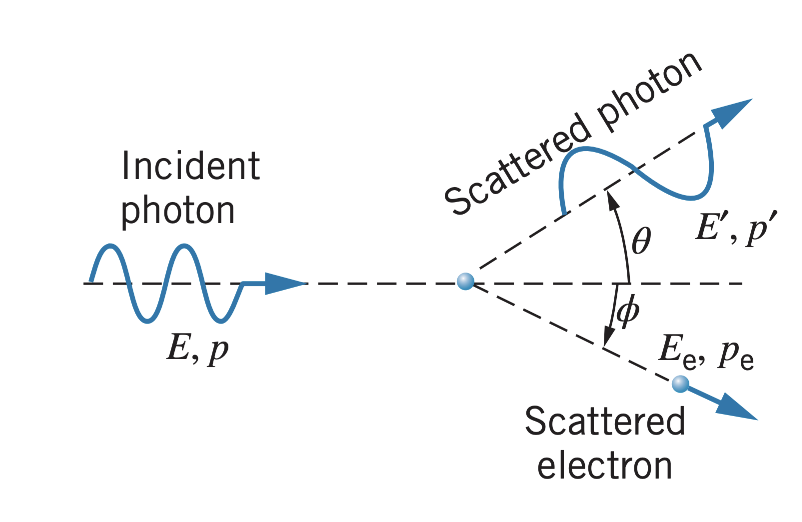
\includegraphics[width=0.4\textwidth]{figures/compton}
	\caption{A schematic diagram of compton process. (Krane, 2020)}
	\label{fig:figures-compton}
\end{figure}

In the Compton scattering experiment, we measure the energy and angle of the scattered photon. We can then test if the measured values satisfy Eq.~(\ref{eq8}). If the measured wavelength of the scattered photon is larger than the incident photon's wavelength, and the measured angle is consistent with the Compton formula, we can confirm that the Compton scattering process has occurred.



\section{Experimental apparatus and procedure}

A setup was employed where photons emitted from an X-ray source collide with a stationary aluminum rod [7]. The scattered photons were then detected by moving detectors positioned at various angles with respect to the incident photons, see Figure \ref{fig:experiment-setup}. The experiment was conducted using a $^{137}$Cs gamma ray source with an energy of 661.7 keV. A NaI(Tl) crystal scintillator was used as the detector, which measured the gamma-ray energies. The detector output was then converted into an electrical pulse proportional to the light's intensity by a photomultiplier tube (PMT) [7].

The photon count spectrum was measured at angles of 5°, 10°, and increments of 10° up to 90°, with measurement uncertainty $\pm 0.5 $°. Photons were accumulated for 3-10 minutes at each angle until the peaks became statistically significant. The centroid of each peak was recorded, along with the angle and the live-time over which data was accumulated. The photon energy was calibrated against the Multi-Channel Analyzer (MCA) channel number, and the angular scale was verified.

To calculate the peak energy, $E_{\max}(\theta)$, the PMT was positioned at different angles, and the photon count spectrum was measured. The peak energy was identified as the principal reflected energy. The change in scattered gamma-ray energy as a function of the scattering angle was then studied to confirm the experimental results with the theoretical predictions given by equation \eqref{eq8}.

The uncertainties in the scattering angle were determined by considering the angular spread of the detector and assuming a uniform spread of photon energy across the detector. The uncertainty was calculated using the standard deviation of a uniform distribution. The uncertainty associated with the peak energy was estimated by measuring the mean and root mean square (RMS) of the distribution of photon energies recorded with the PMT at 5°. The RMS of this distribution was used to estimate the uncertainty on any given measurement. The Monte-Carlo simulation was performed to estimate the uncertainty associated with the value of $m_ec^2$, which took into account the distribution of the slope under Gaussian perturbations of each data point according to their respective uncertainties. For details of slope uncertainty estimation, see Appendix 1.

\begin{figure}[htpb]
	\centering
	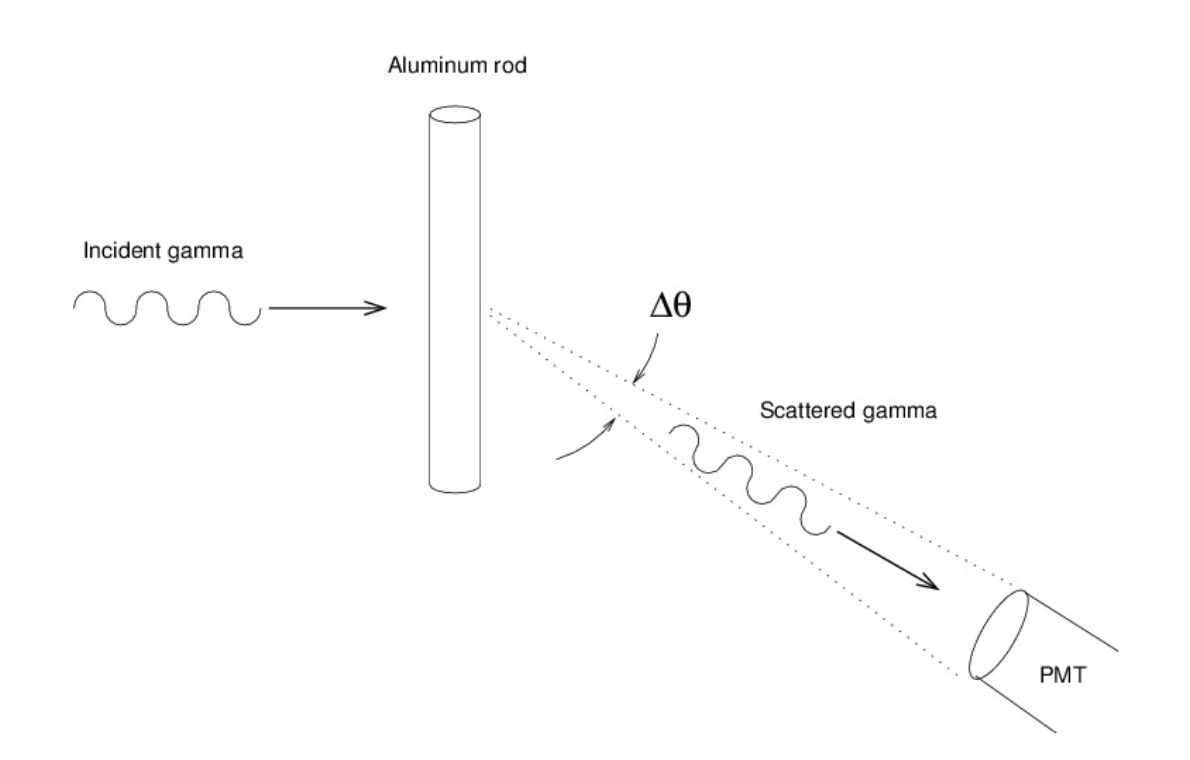
\includegraphics[width=0.8\textwidth]{figures/angle}
	\caption{The experiment set-up. (Lab Manual, 2020)}
	\label{fig:experiment-setup}
\end{figure}

\newpage
\section{Data, analysis, results and uncertainties}

\subsection{Uncertainty Analysis from measurements}

In the experiment, several sources of uncertainty were present, which needed to be identified, analyzed, and estimated for the results' accuracy and reliability.

One source of uncertainty was the scattering angle measurement. Due to the poorly conditioned detector platform, the angular measurements could not be taken accurately. The angular spread of the detector was estimated to be about 0.2°. To estimate the uncertainty, the standard deviation of a uniform distribution was calculated, given by $\sigma^2 = (\Delta\theta)^2/12$, where $\Delta\theta$ represents the angular width of the detector. This estimation method provided an approximate error estimate for the scattering angle measurements.

\begin{figure}[htpb]
	\centering
	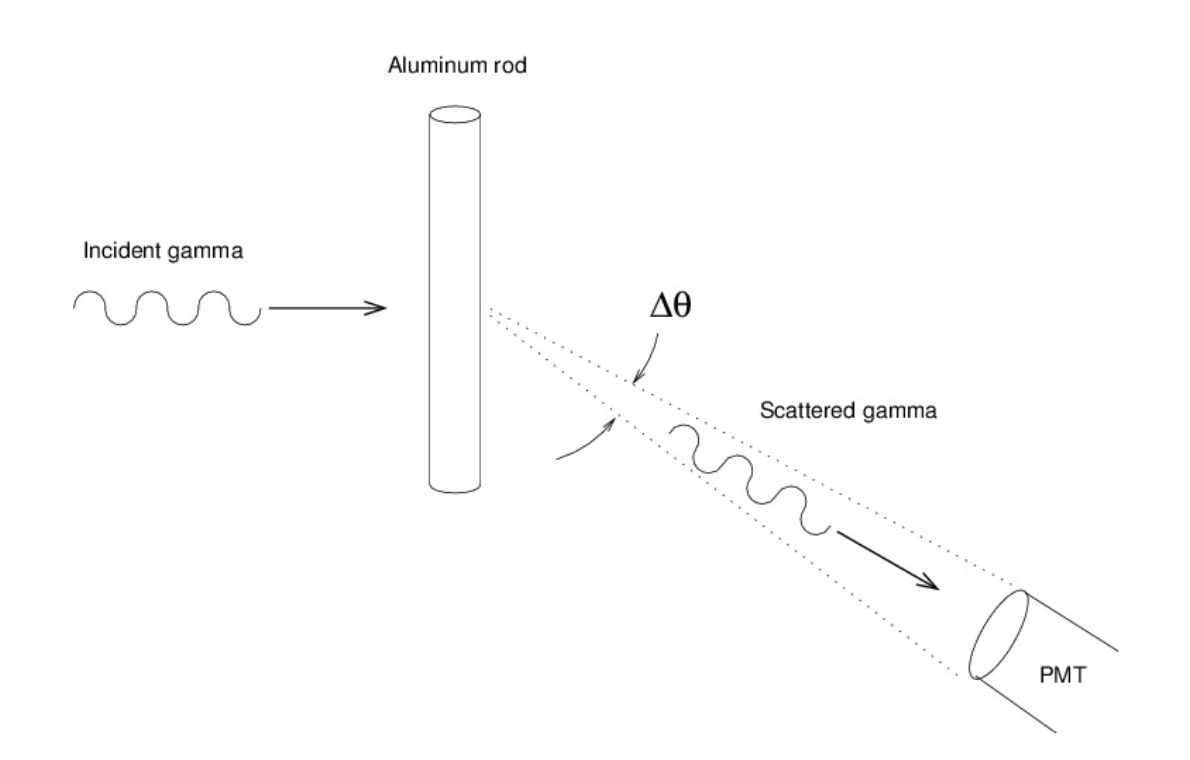
\includegraphics[width=0.8\textwidth]{figures/angle}
	\caption{A schematic diagram of angular calibration process. (Lab Manual, 2020)}
	\label{fig:figures-angle}
\end{figure}

Another source of uncertainty was the peak energy measurement, which could have been influenced by several factors, such as the PMT's gain fluctuations or the background noise. The RMS of the distribution of photon energies recorded with the PMT at 5° was used to estimate the uncertainty on any given measurement, as it reflects the size of any uncontrolled fluctuations in gain. This analysis helped account for possible errors in the experimental data.

The calibration of the energy scale was also a significant source of uncertainty, as it influenced the accuracy of the measured photon energies. The uncertainty in the energy calibration was estimated to be about 0.5 keV, which was determined by the standard deviation of the mean of the calibration points.

\subsection{Data Collection and analysis}

The angles considered for this study are 5°, 10°, and increments of 10° up to 90°. For each angle, photons are accumulated for 3-10 minutes, until the peaks become statistically significant. The detector is positioned at each angle, and the photon count spectrum, $C(\theta, E)$, is recorded with respect to the energy $E$. The live-time over which data was accumulated, the angle, and the measured centroid of the peak are documented for further analysis.

To analyze the collected data, we first observe equation (3), which suggests a linear relationship between $1/E_{\max}$ and $(1 - \cos\theta)$. By calculating these values from the experimental data, we can establish this linear relation and compare it with the theoretical predictions. This comparison helps us understand the consistency of the experimental results with the underlying theory of Compton scattering. For detailed analysis and sample calculation, see Appendix (2).



\subsection{Uncertainty Analysis of peak energy}

To analyze the uncertainty in peak energy, we first measure the mean and root mean square (RMS) of the distribution of photon energies recorded with the PMT at 5°. The RMS of this distribution can be used to estimate the uncertainty on any given measurement, as it reflects the size of any uncontrolled fluctuations in gain. This analysis helps to account for possible errors in the experimental data.

The rest energy of the electron, $m_ec^2$, is determined from the slope of the linear relation between $1/E_{\max}$ and $(1 - \cos\theta)$. To estimate the uncertainty associated with this value, a Monte-Carlo simulation is performed, which takes into account the distribution of the slope under Gaussian perturbations of each data point according to their respective uncertainties. This simulation allows us to obtain a more accurate representation of the uncertainty in the calculated $m_ec^2$ value.

\subsection{Results}

The results of the experiment show a strong linear relationship between $1/E_{\max}$ and $(1 - \cos\theta)$, in agreement with the theoretical predictions. The experimental value of the rest energy of the electron, $m_ec^2$, was determined to be $0.514 \text{MeV}$ with an uncertainty of $ \pm 79 \text{keV}$, which compares well with the accepted value of 0.511 MeV. The uncertainties in scattering angle and peak energy were found to be within acceptable limits, supporting the validity of the experimental findings.

\begin{figure}[htpb]
	\centering
	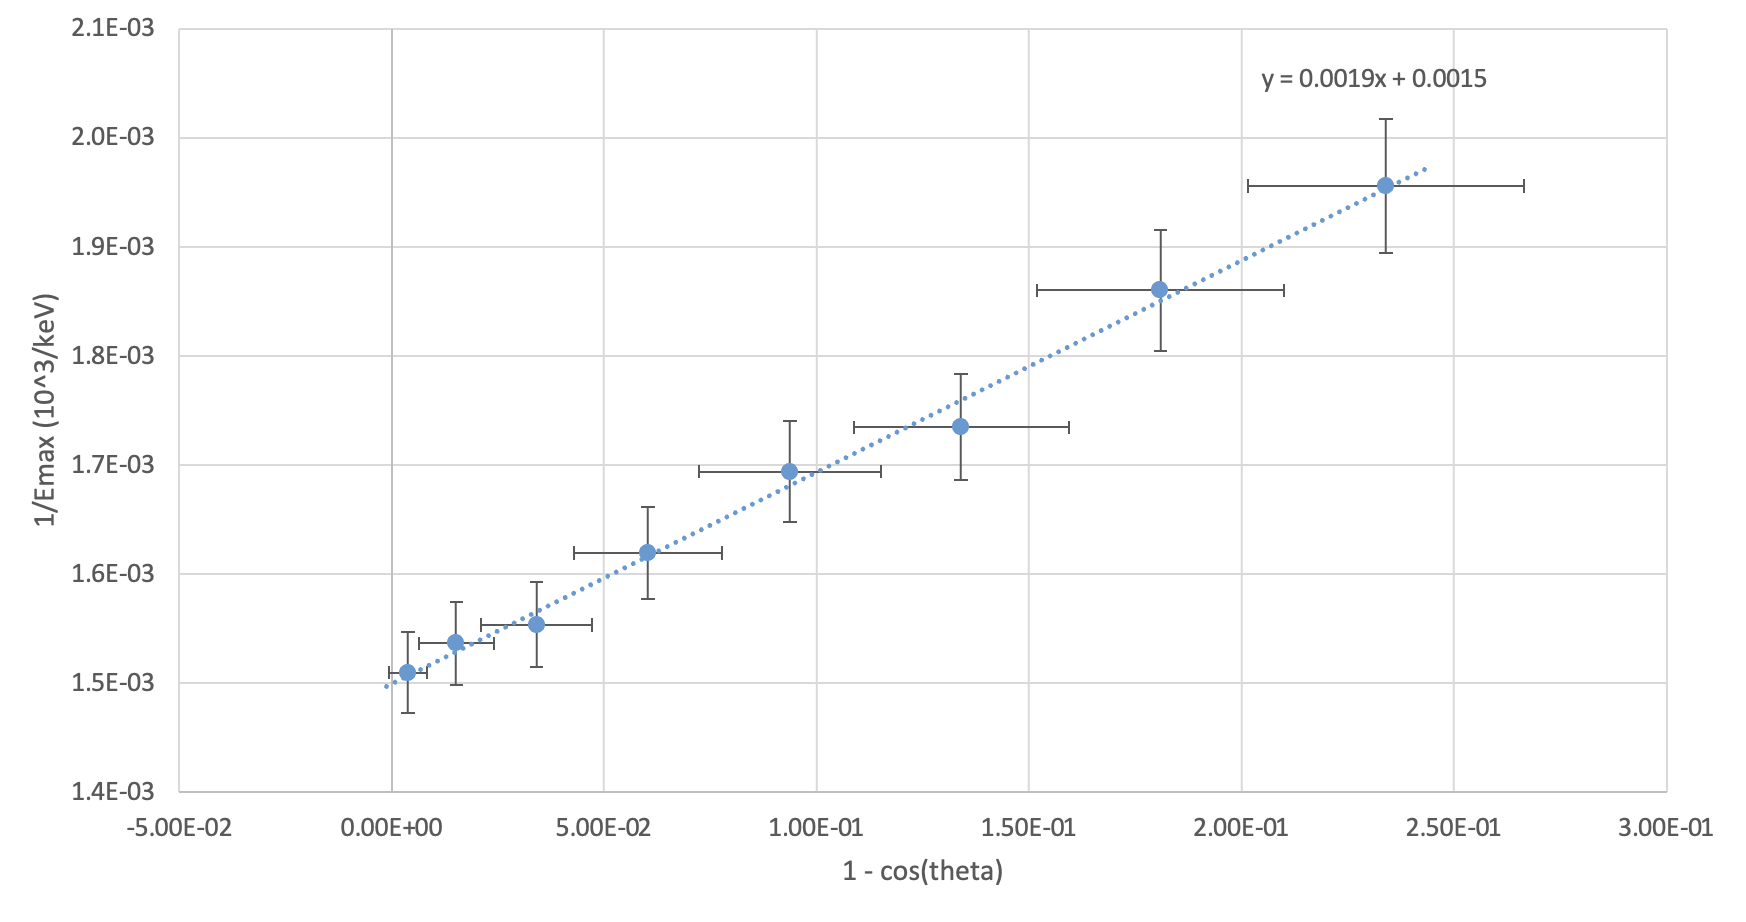
\includegraphics[width=\textwidth]{figures/result}
	\caption{A plot of $(1 - \cos\theta)$ versus $(1/E_{\max})$ for the Compton scattering experiment. A strong linear correlation is observed, in agreement with the theoretical predictions. However, large angular uncertainties are present. }
	\label{fig:figures-result}
\end{figure}

\section{Discussion of results}

The results of our study confirm the linear relationship between $(1-\cos\theta)$ and $(1/E_{\max})$, in agreement with the theoretical predictions derived from the Compton scattering theory. Our experimental determination of the rest energy of the electron, $m_ec^2 = 514 \pm 79$ keV, is within 0.5\% relative error of the accepted value of 0.511 MeV, demonstrating good accuracy and precision of our measurements.

However, our study is not without limitations. One of the major sources of uncertainty in our study is the inability to take precise angular readings due to the poorly conditioned detector platform. This resulted in a large nominal relative error of 15\%, limiting our ability to accurately determine the scattering angles. Additionally, the energy spectra did not include enough samples due to time constraints, generating an approximately 3.5\% relative error of the peak energy.

Despite these limitations, our study provides valuable insights into the interaction between photons and electrons, and the underlying principles of Compton scattering. Our results support the theoretical predictions and could have significant implications for the advancement of our understanding of fundamental particle interactions.

In terms of the theory, our study supports the wave-particle duality concept proposed by de Broglie, demonstrating the particle-like behavior of photons through momentum conservation during collisions. Further studies could focus on refining the measurement process and incorporating more accurate instruments to reduce uncertainties and provide a more precise determination of the rest energy of the electron. Additionally, future experiments could explore the Compton effect in different materials and under various conditions to further refine our understanding of the principles of Compton scattering.

In conclusion, our study provides strong evidence supporting the theoretical predictions of Compton scattering and demonstrates the wave-particle duality of photons. While our study has limitations, the implications of our results on the theory of fundamental particle interactions are significant, and future research could focus on further refining our understanding of Compton scattering and its applications in the study of quantum physics.

\section{Conclusion}

In conclusion, this study of Compton scattering has demonstrated a strong linear correlation between $(1 - \cos\theta)$ and $(1/E_{\max})$, in agreement with the theoretical predictions. Our experimental results support the underlying theory of Compton scattering and provide valuable insights into the interaction between photons and electrons. However, the presence of large angular uncertainties due to the lack of precise instrumentation in locating the detector highlights the need for improved experimental setup and techniques. Future work could focus on refining the measurement process and employing more accurate instruments to reduce these uncertainties. Overall, the successful determination of the rest energy of the electron, $m_ec^2$, along with its uncertainty obtained through a Monte-Carlo simulation, showcases the usefulness of Compton scattering in the study of fundamental particle interactions and the advancement of our understanding of the quantum world.

\section{Acknowledgments}

We would like to express our sincere gratitude to Prof. Ritchie and Prof. Ma for their invaluable guidance and support throughout the course of this experiment. Their expertise in the principles of Compton scattering and their dedication to teaching have been instrumental in our understanding of the subject matter. Without their help, this experiment would not have been possible. 

\section{Bibliography}

\begin{hangparas}{.25in}{1}
[1] A. Einstein, "Über einen die Erzeugung und Verwandlung des Lichtes betreffenden heuristischen Gesichtspunkt," Annalen der Physik, vol. 17, pp. 132-148, 1905.

[2] L. de Broglie, "Recherches sur la théorie des quanta," PhD thesis, Université Paris, 1924.

[3] T. Young, "Experiments and calculations relative to physical optics," Philosophical Transactions of the Royal Society of London, vol. 91, pp. 12-48, 1801.

[4] A. H. Compton, "A quantum theory of the scattering of X-rays by light elements," Physical Review, vol. 21, pp. 483-502, 1923.

[5] Compton, A. H. "A quantum theory of the scattering of X-rays by light elements." Physical Review 21.5 (1923): 715.

[6] Compton, A. H. "The Spectrum of Scattered X-Rays." Physical Review 22.5 (1923): 409.

[7] Melissinos, Adrian C. Experiments in Modern Physics. Academic Press, New York, 1966, pp. 252-265.

[8] Krane, Kenneth S. Modern Physics, 2nd ed., Wiley and Sons, New York, 1996, pp. 83-87.
\end{hangparas}
\newpage

\section*{Appendix 1}
\addcontentsline{toc}{section}{Appendix 1}

\textbf{Monte Carlo method for estimating uncertainty of slope in linear regression with uncertainties in data points}

\begin{enumerate}
\item Start with a set of data points $(x_i,y_i)$ where each data point has its own uncertainties, denoted by $\sigma_i$.
\item Choose a value for the slope of the linear regression line, denoted by $m$.
\item For each data point $(x_i,y_i)$, generate a new data point $(x_i^\prime,y_i^\prime)$ by drawing random values of $x_i^\prime$ and $y_i^\prime$ from normal distributions with means equal to $x_i$ and $y_i$, respectively, and standard deviations equal to $\sigma_i$.
\item Fit a linear regression line to the new set of data points $(x_i^\prime,y_i^\prime)$ using the chosen value of $m$.
\item Repeat steps 3 and 4 many times (e.g., 10,000 times) to generate a large number of linear regression lines based on different sets of randomly generated data points.
\item Calculate the standard deviation of the distribution of slopes obtained in step 5. This represents the uncertainty in the slope due to the uncertainties in the original data points.
\item Optionally, repeat steps 2-6 for different values of the intercept of the linear regression line to estimate the uncertainty in the intercept as well.
\end{enumerate}


\section*{Appendix 2}
\addcontentsline{toc}{section}{Appendix 2}

\subsection{Calibration Process}

The calibration process involved setting the high voltage and pre-amplifier gain so that the 137Cs peak appeared between channels 800 and 900. The spectrum of the 137Cs source was then recorded with the detector seeing direct, unscattered gamma rays, without the Al rod installed. The channel numbers corresponding to the 662 keV gamma ray from 137Cs and the 74 keV K-shell x-ray emission line from Pb were identified, as these two data points were sufficient for determining the two calibration constants in E(keV) = A + BN. The spectrum was saved in TKA file format, suitable for importing into Microsoft Excel. A graph of channel number vs energy (in keV) was plotted for the set of isotope peaks studied, and a straight line and a second-order polynomial were fit to the curve to determine the calibration curve. The calibration was checked by looking for a broader peak near 184 keV in the original spectrum, which was caused by Compton "back-scattered" gamma rays. The Compton formula was used to confirm that the resultant energy should be in this region for $\theta=180$ deg. 

\begin{figure}[htpb]
	\centering
	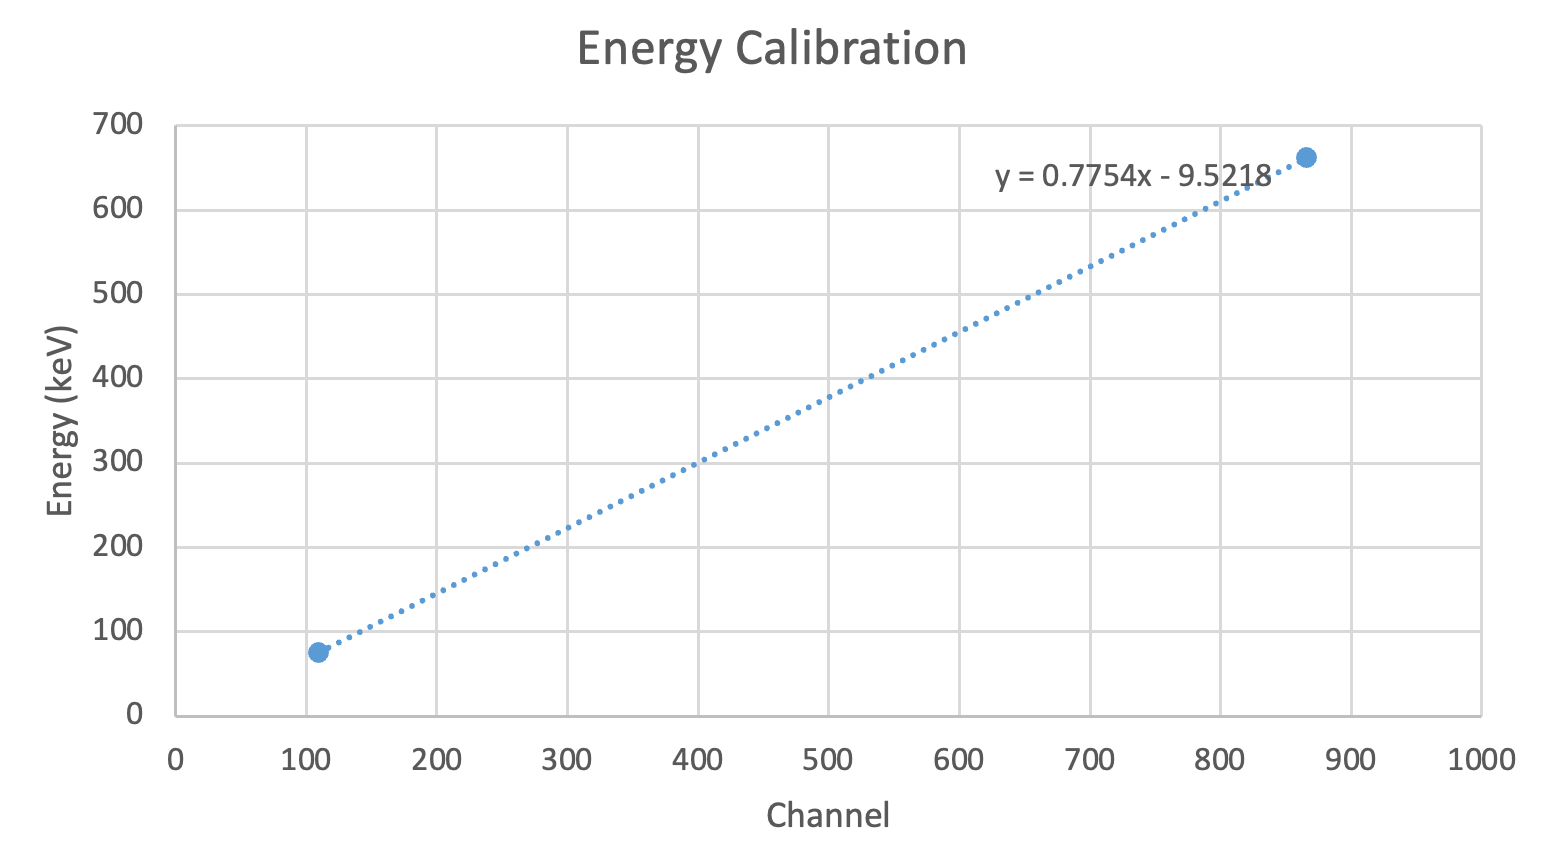
\includegraphics[width=0.8\textwidth]{figures/calib}
	\caption{Calibration diagram.}
	\label{fig:figures-calib}
\end{figure}

\subsection{Data}

The following table summarizes raw data obtained from measurement.
\begin{table}[htbp]
\centering
\begin{tabular}{ccccccc}
\hline
$\theta$ & Centroid & $1-\cos(\theta/180*\pi)$ & $E$ & $1/E$ & Uncer $1/E$ & Uncer $\cos\theta$\\
(degrees) & & & (keV) & (1/keV) & (1/keV) & \\
\hline
5 & 866.4 & 3.81E-03 & 662.28 & 1.5099E-03 & 3.69E-05 & 4.41E-03\\
10 & 851.48 & 1.52E-02 & 650.72 & 1.5368E-03 & 3.82E-05 & 8.79E-03\\
15 & 842.32 & 3.41E-02 & 643.61 & 1.5537E-03 & 3.90E-05 & 1.31E-02\\
20 & 808.67 & 6.03E-02 & 617.52 & 1.6194E-03 & 4.24E-05 & 1.73E-02\\
25 & 773.46 & 9.37E-02 & 590.22 & 1.6943E-03 & 4.63E-05 & 2.14E-02\\
30 & 755.73 & 1.34E-01 & 576.47 & 1.7347E-03 & 4.85E-05 & 2.53E-02\\
35 & 705.53 & 1.81E-01 & 537.55 & 1.8603E-03 & 5.58E-05 & 2.90E-02\\
40 & 671.58 & 2.34E-01 & 511.22 & 1.9561E-03 & 6.16E-05 & 3.25E-02\\
\hline
\end{tabular}
\caption{Experimental data for the scattering angle $\theta$ and corresponding values for the centroid position, $1-\cos(\theta/180*\pi)$, energy $E$, $1/E$, uncertainty in $1/E$, and uncertainty in $\cos\theta$.}
\label{tab:data}
\end{table}






\subsection{Sample Calculation}

We calculate the first row.

Measurements and uncertainties:
$\theta = 5^\circ \pm 2.9^\circ$
$E_{\rm max} = 662.28 \pm 10.57$ keV (where the uncertainty is the FWHM of the centroid)
Convert degrees to radians:
$\theta_{\rm rad} = \theta \cdot \frac{\pi}{180} = 0.0873 \pm 0.0016$ rad

Calculate $1 - \cos\theta$ and its uncertainty:
$1 - \cos\theta = 1 - \cos(0.0873) = 0.00381 \pm 0.00441$

(using the fact that the uncertainty in $\cos\theta$ is given by $\Delta\cos\theta = |\sin\theta|\cdot\Delta\theta$)

Calculate $E_{\rm max}$ and its uncertainty:
$E_{\rm max} = 662.28 \pm 10.57$ keV

Calculate $1/E_{\rm max}$ and its uncertainty:
$\frac{1}{E_{\rm max}} = \frac{1}{662.28 \pm 10.57 \text{ keV}} = (1.5099 \pm 0.0369)\times10^{-3}\text{ keV}^{-1}$

(using the fact that if $x$ has uncertainty $\Delta x$, then the uncertainty in $1/x$ is given by $\Delta(1/x) = |\frac{\Delta x}{x^2}|$)
